\section{Fingerprinting: Value Based Caching}

 Whether an application uses compression or intricate caching mechanisms, the easiest way to improve content delivery speed is to \textit{send less over the network}. With this in mind, a lot of research has been done with respect to protocols focused on eliminating redundant data transfers over HTTP links. Much of this redundancy is caused by the first-class nature of the \lq file \rq in traditional caching systems.\\

\noindent
Inspired by research at Berkley on value based caching\cite{Rhea09}, Flying Squid's Fingerprinting system caches with respect to data, not file name. As a result, only changed and new parts of content need ever retransmitted over a network. 


\subsection{The API}

Flying Squid's value based caching protocol takes the form of a simple, C++ class-based library. Modules exist on both the client and user side, and must be used together.

\subsubsection{Client}

\begin{lstlisting}
class RabinClient
{
    public:
        /* Server name and port number*/
        RabinClient(char * hostname, int port_);
       
	 ~RabinClient();

        /*
        * Receives a file from the server into the open, write enabled file pointer 'file'.
        * Returns the number of blocks added to the file.
	 * This is a blocking call.
        */
        unsigned receive_file(FILE *file); 

       /* Establishes a connection to the server */
        int connect_to_server();

	 /* Disconnects from the server */
        int disconnect_from_server();

};

\end{lstlisting}

\subsubsection{Server}

\begin{lstlisting}
class RabinServer
{

    public:
        /* Port at which to be open*/
        RabinServer(int port_);
        ~RabinServer();

        /* Sends a file of size s to the client.
		This is a blocking call.
	*/
        int send_file(char *file, size_t s); 


        /* Listens for the client and accepts a connection 
        * Must be called before write_to_client is called  */
        int connect_to_client();

	 /* Connects to the client */
        int disconnect_from_client();

};

\end{lstlisting}

\subsection{Integrating Value-Based Caching}

\noindent
Flying Squid uses modified TCP forwarding servers \cite{Partow} at both the client and server sides to interface value-based caching with ATS.

\begin{figure}[H] \centering
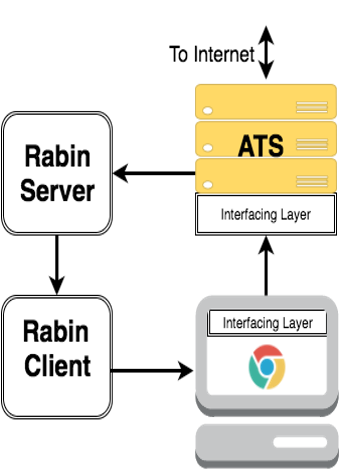
\includegraphics[width=9cm]{FingerprintingArch}
\caption{Flying Squid Value Based Caching Architecture}
\end{figure}

\noindent
When the user makes a request through the browser, the browser forwards the request through its interfacing layer to the interfacing layer of ATS. ATS receives this request and gathers the requested data file from the Internet and the cloud caching mechanism previously described. ATS then sends over the file to the Rabin Server, which breaks down the file into blocks. The Rabin Server sends each block to the Rabin Client, which reassembles the blocks into a file. The Rabin Client then sends the response to the browser through the browser's interfacing layer. Lastly, the browser displays the response to the user. 

\subsection{Technical Approach}

Flying Squid's Rabin Fingerprinting library provides a clean file transfer abstraction to the user, hiding the intricacies of a partial file transfer abstraction.

\begin{enumerate}

\item Server-side files are split into blocks of maximum size $1 KB$ using a \verb|djb-2|\cite{djb2} based uniform random function of the form: \\
$f: \{\text{byte} * \text{byte} * \text{byte} \} \rightarrow \{0, 1, ..., 1023\}$
 
\item Block boundaries are determined when this function returns 0. These blocks are treated as first-class objects and are hashed locally. A custom protocol can then be used to transfer the blocks representing a file over a TCP connection. Only the hash digests (identifiers) of previously transmitted blocks are transferred. Blocks of size 0 are used to denote $EOF$.

\item The client  leverages the ordering properties of TCP to receive blocks in order. These are then locally stored, and identifiers are used to re-assemble them into traditional files. 
\end{enumerate}

\subsection {Statistics}

Pairs of files were generated that differ in the following ways:

\begin{enumerate}
\item Haskell: One file has an added byte.
\item HTML: Files differ by one large contiguous chunk.
\item C: Files differ by a large number of chunks distributed through the file
\end{enumerate}

For each pair, these pairs of files were sent one after the other over a network using the Flying Squid fingerprinting system, with different maximum block sizes. Max block sizes 	smaller than $256$ bytes were found to cause significantly more conflicts with the internal \verb|djb2| hash. 


\begin{figure}[H] \centering
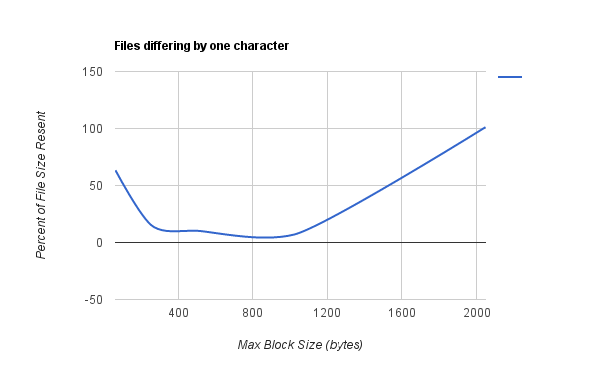
\includegraphics[width=\textwidth]{HaskellGraph.png}
\caption{Details the percent of the second file sent at different max block sizes.}
\end{figure}
\noindent
For files differing by one byte, a balance has to be struck between several small block headers being sent and the size of the retransmitted block(s). At most one block will be retransmitted due to the small difference between files. An optimal block size was found around $1000$ bytes

\begin{figure}[H] \centering
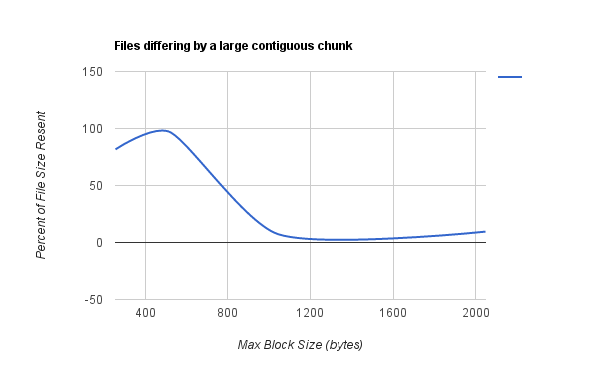
\includegraphics[width=\textwidth]{HTMLGraph.png}
\caption{Details the percent of the second file sent at different max block sizes.}
\end{figure}
\noindent
For files differing by a large contiguous chunk a minimum was found around $1400$ bytes.

\begin{figure}[H] \centering
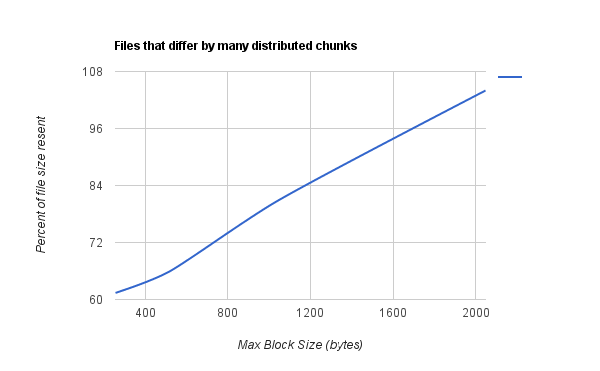
\includegraphics[width=\textwidth]{CGraph.png}
\caption{Details the percent of the second file sent at different max block sizes.}
\end{figure}
\noindent
For files differing by a large number of chunks distributed through the file, smaller max block sizes were generally found to be better.


\begin{figure}[H] \centering
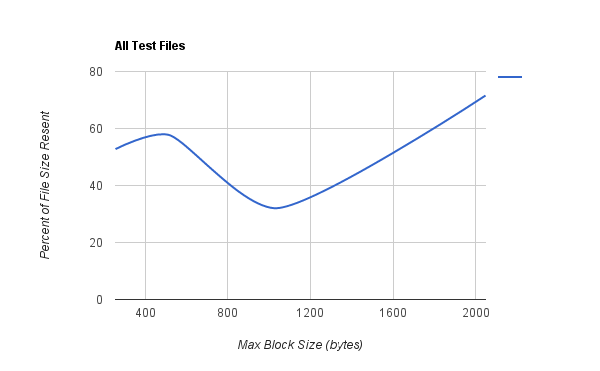
\includegraphics[width=\textwidth]{AllGraph.png}
\caption{Details the percent of the second file sent at different max block sizes.}
\end{figure}
\noindent
Taking the average of all these files, it was found that a minimal amount was resent around a maximum block size of $1 KB$. As a result, the maximum value chosen was $1024$ bytes, with an expected max size of $512$ bytes.
